\section{Build system}
\begin{frame}[t]
	\center{\huge{Construire son système}}
	\begin{figure}
		 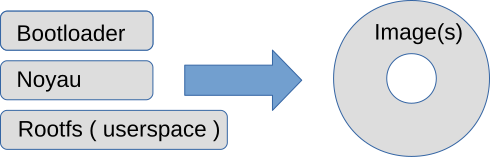
\includegraphics[height=1.5cm]{img/build.png}
	\end{figure}
	\vspace{-1.1cm} % #propreté
	\begin{columns}[t]
	\begin{column}{0.45\textwidth}
	\uncover<2->{\center{Non merci !}}
	\begin{block}<3->{Distribution classique}
		\begin{itemize}
			\item Simple
			\item Pas flexible
			\item Pas optimisé
			\item Architectures classiques
		\end{itemize}
	\end{block}
	\end{column}
	\begin{column}{0.45\textwidth}
	\uncover<4->{\center{Trop facile !}}
	\begin{block}<5->{À la main}
		\begin{itemize}
			\item Flexible
			\item Pas reproductible
			\item Pas maintenable
			\item Pas de dépendances
		\end{itemize}
	\end{block}
	\end{column}
	\end{columns}
\end{frame}
\begin{frame}
	\center{\huge{Build system}}
	\begin{itemize}
		\item<1-> Configure, construit et package les composants
		\item<2-> Gère les dépendances
		\item<3-> Permet la reproductibilité
		\item<4-> Génère la chaine de cross-compilation
	\end{itemize}
\begin{block}<5->{Choix critique}
	\begin{itemize}
		\item<6-> Conditionne le développement
		\item<7-> Conditionne l'évolution du projet
		\item<8-> Conditionne les livrables
	\end{itemize}
\end{block}
\end{frame}
% schema
\subsection{Buildroot}
\begin{frame}
	\center{\huge{Buildroot}}
	\begin{columns}
		\begin{column}{0.65\textwidth}
			\begin{itemize}
				\item<1-> Makefiles, Kconfig
				\item<2-> Rootfs, Bootloader, Kernel, Toolchain
				\item<3-> Répandu et simple d'utilisation
				\item<4-> 1 carte = 1 buildroot
			\end{itemize}
		\end{column}
		\begin{column}{0.30\textwidth}
			\begin{figure}
				 \includegraphics<1->[height=2cm]{img/buildroot.png}
				 \uncover<1->{\caption{Logo buildroot}}
			\end{figure}
		\end{column}
	\end{columns}
	\begin{block}<5->{Pourquoi Buildroot ?}
		\begin{itemize}
			\item<6-> Cartes sans variantes
			\item<7-> Prototypage
			\item<8-> Projet "Simple"
		\end{itemize}
	\end{block}
\end{frame}
% buildroot
\subsection{Yocto}
% yocto
\begin{frame}
	\center{\huge{Yocto project}}
		\begin{itemize}
			\item<2-> Groupes de composants réutilisables : Layers
			\item<3-> Scripts surchargeables : Recipes
			\item<4-> Grosse base de composants
			\item<5-> Rootfs, Kernel, Bootloader, Toolchain, Paquets
			\item<6-> Difficile à prendre en main
		\end{itemize}
	\begin{block}<7->{Pourquoi Yocto ?}
	\begin{itemize}
		\item<8-> Gros projet
		\item<9-> Cartes avec variantes
		\item<10-> Favoriser la réutilisation
	\end{itemize}
	\end{block}
\end{frame}

\begin{frame}[t]
	\center{\huge{Yocto c'est simple}}
	\begin{figure}
		 \includegraphics<2->[height=5.1cm]{img/yocto.png}
		 \uncover<2->{\caption{\tiny{http://www.yoctoproject.org/docs/2.1/mega-manual/mega-manual.html}}}
	\end{figure}
\end{frame}

\begin{frame}[t]
	\center{\huge{Yocto c'est simple ( en vrai )}}
	\begin{columns}
		\begin{column}{0.45\textwidth}
			\begin{figure}
%				 \includegraphics<2>[height=3cm]{img/metas.png}
%				 \includegraphics<3>[height=3.1cm]{img/metas_zoom_1.png}
%				 \includegraphics<4>[height=3.2cm]{img/metas_zoom_2.png}
				 \includegraphics<5>[height=3cm]{img/metas_zoom_b12.png}
			\end{figure}
		\end{column}
		\begin{column}{0.55\textwidth}
			\begin{itemize}
				\item<2-> Layers : Base + custom
				\item<3-> Recipes : Comment construire un paquet ?
				\item<4-> Recipes : Possibilité d'extension
				\item<5-> Machine : Layers + Recipes
			\end{itemize}
		\end{column}
	\end{columns}
\end{frame}
